

For example, the class (is, married) should especially to sethe assumption was that sentences containing words such as "married", "spouse" or "single" would help in rating the class (type\_of\_union, marriage)

The Texter is essentially a multi-label classifier with a fixed number of sentences as input and the most common facts, or more precisely, the most common relation-tail tuples that form facts together with the query entity as the fact's head, as its output classes. Figure~\ref{fig:4_approach/1_texter/2_attention_model/texter_architecture} sketches the basic idea of the classifier: Given some sentences about the query entity one, multiple or none of the relation-tail tuples are predicted.

Although it would be desirable to predict any kind of facts that appear in the training data, the output classes are limited to the most common ones to prevent two major problems: First, it would be difficult to counter the impact of the extreme class imbalance between the most and least common classes, leading to overfitting and ineffectiveness, respectively. Second, the increase in learnable parameters would further facilitate overfitting and lead to longer training and inference times. In practice, however, the effects of limiting the output classes are negligible as most relation-tail tuples $(rel \in Relations, tail \in Entities)$ from the theoretically vast domain $Relations \times Entities$ never occur. For example, relation-tail tuples such as $(speaks, actor)$ never occur, limiting the number of reasonable classes and thereby increasing the share of the fixed number of top classes. Furthermore, rare classes can still be predicted by the Ruler.

At a closer look, the Texter consists of an embedding layer, an attention layer, the actual classification layer and a \lstinline{predict()} function. Figure~\ref{fig:common_attention_architecture} shows the three layers which contain all of the model's learnable parameters. The embedding layer receives the query entity's sentences, embeds each one, and passes the sentence embeddings on to the attention layer. The attention layer uses internal \emph{class embeddings} to produce class-dependent entity embeddings that primarily represent the sentences most relevant for the respective class. Those entity embeddings are then passed to the classification layer that pushes the entity embeddings through simple perceptrons, producing the output logits. The three layers are implemented together in the model's \lstinline{forward()} function that also returns the information on which sentences influenced which logits in addition to the logits themselves. That extra information is later used in the \lstinline{predict()} function to rank the facts by relevance for each class.

\begin{figure}[t]
    \centering
    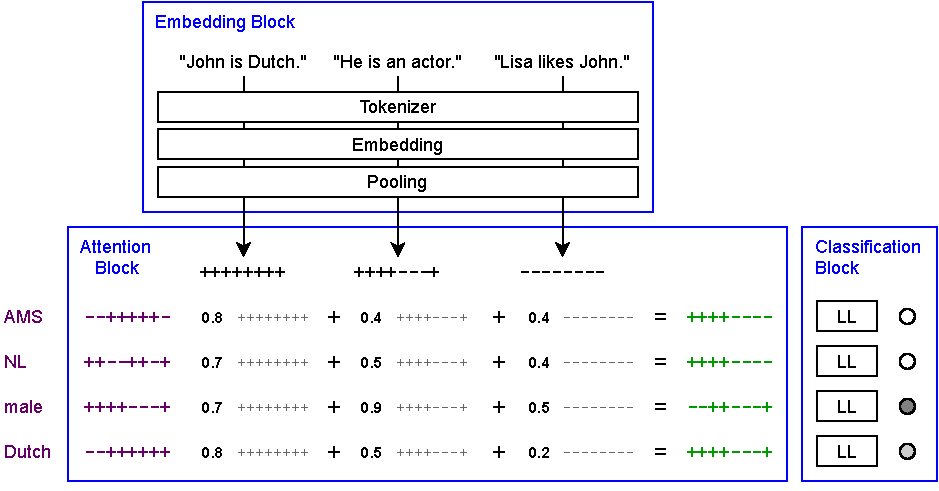
\includegraphics{4_approach/1_texter/2_attention_model/attention_architecture}
    \caption{Texter Architecture}
    \label{fig:4_approach/1_texter/2_attention_model/attention_architecture}
\end{figure}

A walk through the forward phase shows the inner workings of the layers: Starting with the query entity's sentences, a tokenizer splits the sentences into tokens, the tokens are embedded, and the resulting token embeddings are combined to a sentence embedding that represents the sentence as a whole. There are multiple possible ways of choosing a tokenizer, embedding the tokens and combining the token embeddings, some of which are covered in chapter~\ref{ch:5_experiments}. The POWER model's Texter embeds the tokens using DistilBERT~\cite{Sanh2019DistilBERTAD}, a variant of the popular BERT transformer encoder. The DistilBERT model has been pre-trained before and is fine-tuned on the POWER dataset. The tokenizer must match the one used during pre-training - a byte pair encoding tokenizer in the case of DistilBERT - whose vocabulary is only extended by two special tokens that allow marking mentions of the entity within the sentences so that DistilBERT can better understand how the sentence relates to the entity. Finally, the embedding layer produces the sentence embeddings by averaging the respective token embeddings and passes them on to the attention layer.

The attention layer determines which sentences a class attends to and creates the class-wise entity embeddings that focus on the sentences the respective class attends to the most. To do so, the attention layer keeps track of learnable class embeddings that represent the classes and that have the same embedding dimension as the sentence embeddings. Each of the $n_c$ class embeddings $c_i$ is scalar multiplied with each of the $n_s$ sentence embeddings $s_j$ resulting in the \emph{attention matrix} $A$ whose values specify how well a class embedding matches the respective sentence embedding. If class and sentence embeddings are similar, the scalar product gives a positive value, if they are opposite, it gives a negative value, and if similarity and opposite balance out, it gives a value close to 0. Subsequently, the sigmoid function $S$ is applied to the matrix' values, as formulated in~\ref{formula:sigmoid_attention}, mapping them to range $(0, 1)$. Formula~\ref{formula:ent_emb} describes how the attentions values are then used to calculate a weighted sum of the sentence embeddings for each class, resulting in the class-dependent entity embeddings $e^i$ returned by the attention layer.

\begin{align}
    A_{ij} = S(\langle c_i , s_j \rangle) && i \in [1, n_c], j \in [1, n_s]
    \label{formula:sigmoid_attention} \\
    e^i = \sum_{j = 1}^{n_s} A_{ij} \cdot s_j && i \in [1, n_c], j \in [1, n_s]
    \label{formula:ent_emb}
\end{align}

In the classification layer, the class-dependent entity embeddings are forwarded through single-layer, single-output perceptrons whose outputs make up the multi-label output of the model's \lstinline{forward()} function. Given the entity embedding $e^i$ for the ith class, the output logit $y^i$ is calculated as $y^i = w^i \cdot e^i + b^i$, with $w^i$ and $b^i$ being the perceptron's weight vector and bias, respectively. Besides the perceptron's logits, the \lstinline{forward()} function also returns the attention matrix $A$, allowing the \lstinline{predict()} function to rank the importance of the sentences for each class during inference.

Taken together the three layers contain all the Texter's learnable parameters. In total, DistilBERT's $d = 768$ dimensional token embedding for each of the $n_t \approx 30,000$ tokens, the $n_c$ same sized class embeddings and the $n_c$ perceptrons' weights and biases sum up to $n_t \cdot d + n_c \cdot d + n_c \cdot (d + 1)$ parameters. During training, a binary cross-entropy loss function calculates the loss from the sigmoid of the classification logits, matching the underlying multi-label classification task. The gradients calculated during backpropagation are applied by an AdamW optimizer, a variant of the Adam optimizer that overcomes Adam's that keeps the training speed of Adam while keeping SGD's superior ability to generalize~\cite{Loshchilov2019DecoupledWD}.

During inference, all classes above a confidence threshold - 0.5 by default - are predicted to be true. The facts are formed by combining the query entity as head with the relation-tail tuples that make up the classes. The facts ranked by confidence and further supplemented with the sentences that led to their prediction, in the order of relevance as specified by the attention matrix, providing the user with an explanation for the fact predictions.
